%Cloud-Computing Basics a Non tech. intro.
%Seite 163
% Wie werden die Informationen die Benutzer gezeigt und wie können sie diese manipulieren
\paragraph{}

\subsection{Cloud-Dienste, bei deren Geld verschwendet wird}
Ist dieses Kapitel sinnvoll?

\subsection{Optimierungsmaßnahmen}

%auto Scaling  
\subsubsection{Auto Scaling Group }
%https://youtu.be/qYHR_V1lvNU?t=900
Auto Scaling ist es hilfreich, um die richtige Anzahl von EC2 Instanzen zur Verfügung zu haben, um die Anwendungslast abzudecken.
\\\\
Folgende Abbildung zeigt das Verhältnis von einer Anwendung über eine Woche ohne Auto Scaling.
Die graue Zone entspricht ungenutzte Kapazität einer EC2-Instanz. Dies bedeutet, es wird für ungenutzte Ressourcen bezahlt.
\begin{center}
    %TODO: selbst das Bild zu erzeugen, um eine bessere Qualität zu bekommen
    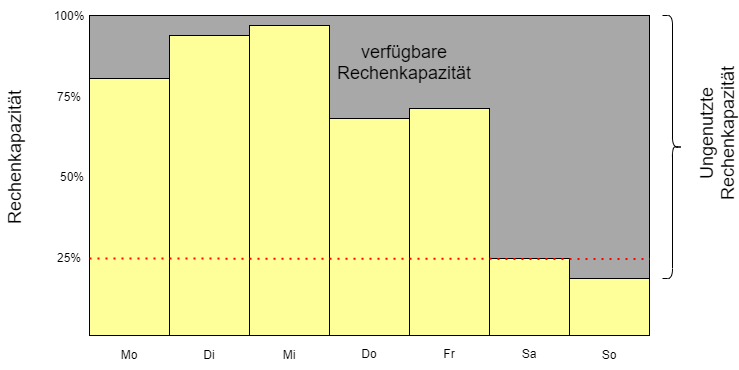
\includegraphics[scale=0.7]{sources/AutoCap Unused Capacity}\label{fig:AutoSca_Unused_Capacity}\\
    \textbf{Abbildung \autoref{fig:AutoSca_Unused_Capacity}:} Ungenutzte Ressourcen
    \footnote{Vgl. u.a.\cite{AMZ01}}
\end{center}


\textbf{Cloud Watch}\\
Amazon CloudWatch ermöglicht die Überwachung der Leistung von Diensten. Es ist relevant für DevOps-Manager, Ingenieure, Entwickler und mehr. Dieses Tool sammelt operative Daten für die Analyse und Entscheidungsfindung.
%(How to use Spots and on-demand)

\subsubsection{Maßnahme: Automate Dev/Test Umgebungen Elasticity}
Grund: Einfach weil kein Entwickler arbeitet 24/7 oder am Wochenende
%Wann ist es sinnvoll Systeme runterzufahren 

\subsubsection{(auto) Tiering }
Grund: nicht alle Dateien brauchen eine höhe Verfügbarkeit
%Tiering, aber automatisch

\subsubsection{Automatisierung mit Lambda Funktionen}
Grund: einmal programmiert, funktioniert es für immer

\subsubsection{Benachrigungen, wenn x\% Kapazität unterschreiten wurde}
Grund: um relevante Ereignise nicht zu verpassen und rechtzeigtig Maßnahmen zu ergreifen
%Limitierung 
%Quotas setzen? erweitern oder reduzieren / benachrichtigen aber auch eine Aktion durchführen 

%Turning stuffs OFF
%Lambda
%Data Pipeline
%CloudWatch

%Economic Performance?
%QUEUES

%NEVER forget your avaliabity requirements, trying to optimize, first availability THEN cost...
%Do not use your DB for saving BLOB
  